\chapter{Result}\label{cha:Research}
%

% Ska följa som ett naturligt komplement till huvuddelen

In this chapter, the results are presented, so that in the next chapter, these results are analysed.

%\section{Example}\label{sec:research:history}
%
Liksom \citep{Duck:2005} har vi kommit fram till att glass smakar bäst på sommaren \citep{Khalil02NonlinearSystemsBook}.

\marginpar{Kommer att tänka på en liten anekdot\ldots}

\Warning[TODO]{Ta bort den löjliga anekdoten!}

\begin{figure}[tbp]
  \centering
  \subfloat[Alldeles för tidigt.][\label{fig:times:very-early}Det här är väl tidigt — din glass hinner smälta innan ditt sällskap dyker upp.]{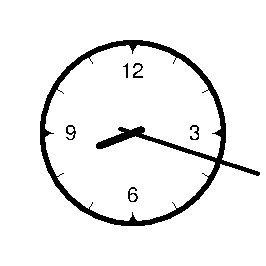
\includegraphics[page=1]{clocks}}
  \qquad
  \subfloat[Med marginal.][\label{fig:times:early}Kiosken stänger snart, men inte nu — perfekt!]{\includegraphics[page=2]{clocks}}
  \\
  \subfloat[I grevens tid.][\label{fig:times:on-time}Precis i tid — du får in ett finger i luckan just när kiosken ska stänga.  Han som jobbar blir sur, och det blir smolk i bägaren.]{\includegraphics[page=3]{clocks}}
  \qquad
  \subfloat[Försent.][\label{fig:times:late}Du är sen — kiosken är stängd.]{\includegraphics[page=4]{clocks}}
  \caption{\label{fig:times}%
    Illustration av \emph{subfloats}.  Den så kallade \emph{bounding box}en visas i \protect\subref{fig:times:late}.  Lägg märke till att bounding boxen har satts så att alla bilder har samma storlek, med enhetlig placering av själva innehållet i förhållande till bounding boxen.  Antag att du ska träffa en kompis för att äta glass just när kiosken stänger för dagen vid 08:30.  När dyker du upp?}
\end{figure}

\section{Developed Application}

Here the results from the app for iteration 2, 3 and 4 are shown. Iteration 1 is missing, as the app development had not started.

\subsection{Iteration \#2}

%Result

\subsection{Iteration \#3}

%Result

\subsection{Iteration \#4}

%Result

\todo{Show images of final app - on mobile, tablet and desktop?}

\section{Qualitative Data}

Here the results from the qualitative data for iteration 1, 2, 3 and 4 are shown.

\subsection{Iteration \#1}

%What the observations said

\subsection{Iteration \#2}

%What the observations said

\subsection{Iteration \#3}

%What the observations said

\subsection{Iteration \#4}

%What the observations said

\section{Quantitative Data}

Here the results from the quantitative data for iteration 1, 2, 3 and 4 are shown.

\subsection{Iteration \#1}

%What the data said

\subsection{Iteration \#2}

%What the data said

\subsection{Iteration \#3}

%What the data said

\subsection{Iteration \#4}

%What the data said

\chapter{Analysis}

% Important to be objective
% En diskussion om hur resultaten kan användas i praktiken är också i de flesta fall belysande och relevant i rapporter

% https://liu.se/ias/kontakta-oss?l=en

In this chapter, each step of the visualization pipeline is presented, allowing analyzing the data. Then, conclusions are presented.

The Visualization Pipeline describes the process of generating an image from the data: \cite{timo-ropinski-liu}

\begin{enumerate}
\item Data acquisition ($\,\to\,$data are given)
\item Data enhancement ($\,\to\,$ data are processed)
\item Visualization mapping ($\,\to\,$ data are mapped to for example a geometry)
\item Rendering (3D->2D) ($\,\to\,$ images generated)
\end{enumerate}

% Timo Ropinski, Scientific Visualization Group, Linköping University, TNM067 - Scientific Visualization, 9/12/2014)
% https://drive.google.com/drive/u/0/folders/0BzlK1PD8EE75bHIxcXRQNWpRMm8

\section{Data acquisition}

This section presents how data was acquired.

\subsection{App usage}
The app pushes data to server when online (it saves quiz start, and quiz finish).

The server receives JSON data, stored in a MongoDB database.

Each data point is saved in a database called Results, with the signed in user (from the Users database).

It was desired to store the data in Google Sheets, thus it was necessary to convert the JSON format into a Google Sheets-readable format, like CSV.

Multiple approaches were tried, and the Google Chrome extension called Magic Json by agaze\_dev\_team (last updated October 29, 2015) %https://chrome.google.com/webstore/detail/magic-json/cajifcebjiflndefndbnoeenjpiiiagm?hl=en
was the one that worked without problems. \cite{agaze}.

\subsection{Pre-study}

The Pre-study data was done by manually recording the paper-submitted pre-study evaluation form from the coaches, into Google Sheets.

\section{Data enhancement}

This section presents how the data was processed, to enable visualization mapping.

\subsection{App usage}
To make the data easier to work with, the columns were reordered, and made sortable and filterable.

Some columns were given conditional formatting, so it would be easier to spot irregularities.

\todo{Lägg till bild "results-colored.png" (finns på skrivbordet)}

After this, some observations could be made. For example, there was a surprisingly low number of answers where the user answered the question without confidence. Also, more users had started a quiz without finishing it than anticipated. Finally, a lot of users had done quizes that were not Topic quiz 3 and Coach quiz 9, which might indicate high interest (if they did more than 2 quizes) or confusion (if they did not do 3 or 9, but they did do other quizes) during the app evaluation. This meant that on some aspects, there were less data than anticipated, (which was troublesome, as there were already few data points), and some aspects where there was more data than anticipated (that were overlooked)

\subsection{Pre-study}
To see differences in answers more clearly, the data from the pre-study was made sortable and filterable. Then, the data was resampeled for each column that hade numerable (sortable) data in text instead of numbers, so e.g. "The day before" was changed to -1 and "The same day" to 0. In a similar way, school level was divided into four different groups, from 0 to 3, where 0 meant secondary, year unknown, 1 meant lower secondary, 2 meant upper secondary, and 3 meant tertiary.

After this, each column was given conditional formats using a color scale, using Google Sheets built-in functionality. This gave a visual way to quickly get a overview of the pre-test data.

Observations from the data was that a surprising number of cells were left blank. One user had not done the pre-test, where some had left questions unanswered (most commonly "Do you own a company?" (should have used the word "business"), plus "Hours of preperation" and "Occations for a youth session" (there is a tendency this might be because they were not proud of their answers, because of correlations with low quiz results).

Missing cells was not as obvious with the app results, were users could not progress in a quiz without answering both the question and the confidence. However, none of the passed quiz 9 certification answers had been submitted. Thus, it was needed to add these from the manual recordings, which had been used as a backup in case anything like this would happen.

\subsection{Summary of app results}

To compare the test results with the pre-test results, it was clear that it would not be viable to test every dimension against every dimension.

Instead, since goals of the app evaluation had been predefined in the following way, the quiz results were summarized so that the following could be derived:

\begin{itemize}
\item \% correct 1st try
\item number of tries until 100\%
\item number of tries until 100\% in 1 try
\end{itemize}

These could be calculated by having columns for:

\begin{itemize}
  \item Quiz 3
  \begin{itemize}
    \item Start time training
    \item \% correct 1st try
    \item number of tries until 100\% in 1 try
    \item Time difference start to end time certification
  \end{itemize}
  \item Quiz 9
  \begin{itemize}
    \item Start time training
    \item \% correct 1st try
    \item Time difference start to end 1st try
    \item Time difference start to passed training
    \item Time difference 1st try to certified
  \end{itemize}
\end{itemize}

Then, to see trends, I again added color scales. With ordinal values, a sequential color scheme is used (e.g. fastest time, from green to red), and with nominal values (like if they are female or male) where there is no right value, a qualitative color scheme is used. Now, it was easier to spot outliers and trends.

First-hand observations were that there was a strong corrolation between pre-quiz results and quiz 9 try 1 (slightly visible also in quiz 3 try 1, but with more outliers). Also, with manuals there was a higher probability to finishing quiz 9 training + certification. More

\subsubsection{Comparing the pre-test and results summary sheets}

I joined the two sheets, meaning I had created a multiple-variate data set (serveral dimensions that I needed to compare with several dimensions).

I met with my university supervisors, so they could further support me in how to properly analyze the data.

It was clear that analysis in Google Sheets could only go so far. It was greatly helpful to sort by multiple columns (e.g. first by Manual?, then by School level, then by Quiz 3). However, it took a long time to filter the data on multiple parameters, and the work became tedious. It was not viable to discover the data using this approach.

Meeting with the supervisors, they started by comparing the means on the pre-quiz results with the two control groups. Since they showed similar results, the two control groups were comparable.

Then, we calculated the means from the other columns based on e.g. "Manual?", gender, school category, high app quiz result, etc.

A multivariate analyzation software or a visualization was suggested to discover the data in less time.

It was hard for us to determine a suitable multivariate analysis software suitable when having so few data points. Principle Component Analysis or Cohen's kappa would not be suitable, or to do Linear correlation on all dimensions.

After discussion with other Master thesis students working with large amounts of data (one from KTS and one from MT), parallel coordinates was suggested. It would allow me to very quickly filter the data, find correlations, and distinguish outliers and common characteristics.

To learn how to analyse the data, Une-terre (2012) was consulted. % http://une-terre.blogspot.se/2012/09/parallel-coordinates-read-out-patterns.html
He writes "||-coords are a data visualisation which allow you to "read out" the relationships and trends between your dimensions. Positive relationship (correlation), negative relationship (invert), or no relationship (random)."

\subsection{Visualization mapping}
The goal with visualization mapping is to generate renderable data.

Thus, I added a new spreadsheet, specific for visualizing the data.

I deleted columns that would serve no visual purpose (e.g. timestamps), gave all cells data values (even N/A when undefined), deleting users that did not have data, and shortened the column names so they would fit on the screen.

The data was then exported from the Google Sheet into CSV.

\subsection{Rendering}

For rendering, the JavaScript library D3.js was chosen. It supports data-driven documents for visualizing data with HTML, SVG and CSS. It supports both JSON and CSV data.

A visual framework for multidimensional detectives for D3.js was found, called "Parcoords.js", written by Chang Kai (2012).
% https://syntagmatic.github.io/parallel-coordinates/
% Chang, K. (2012). Parallel Coordinates toolkit : Parcoords.js 0.1. Parallel Coordinates toolkit. Retrieved September 8, 2012, from http://syntagmatic.github.com/parallel-coordinates/
% Kosara, R. (2010, May 13). Parallel Coordinates. Eagereyes.org. Retrieved September 8, 2012, from http://eagereyes.org/techniques/parallel-coordinates
% Tricaud, S. (2008). Picviz: finding a needle in a haystack. Proceedings WASL, San Diego. Retrieved from http://www.usenix.org/events/wasl08/tech/full_papers/tricaud/tricaud.pdf

The example code from "Linking with a Data Table" provided the basis for the rendering. It would be a great benefit to bee able to see both a parallel coordinates visualization, and to see the same values present in the Google Sheet. %https://syntagmatic.github.io/parallel-coordinates/examples/table.html

I replaced the example CSV file with the exported Google Sheets data in CSV.

Eventually, I also changed the colors, and added to the example the toolkit's functionality to drag the axes titles around to reorder the dimensions, since the goal was to quickly compare and find correlations.

\todo{Lägg till bild på parallella koordinater-visualiseringen}

\section{Findings}

In this section, the conclusions from the different group characteristics are presented.

\subsection{Correlations}

\textbf{Youth mentor (brun), 6 st vs. CBT (blå), 14 st}
* Youth mentors has higher school level than CBT's
* 1/6 Youth mentors had brought manual, compared with 8/14 CBT's
* Only 1 CBT has above 2 (1 st 3) on School, while YM have (2st 0, 1 2st, 2 2st)
* Inverse correlation: CBT old, YM young
* There are no female Youth Mentors (i.e. 100\% male Youth Mentors)
* All of the YM's run their own businesses, compared with 5/10 for CBT's
* Only CBT's said they didn't feel comfortable with smartphone (2 st) - because of age?
* Seemingly no difference CBT vs. YM in when prepares for session
* All YM prepares 2 times for session, while CBT can train also 3 or 1 time)
* 13/14 CBT's gjorde quiz 3 try 1, 6/6 YM's
* YM's och CBT's presterar lika på quiz 3 try 1
* CBT 6/14 st certifierade, YM 4/6 st

Quiz 9 (rött=CBT:
* 6 CBT's gör ej Q9 try 1, 2 YM gör ej
* YM är top performers på Q9 try 1 jämfört med CBT's
* endast 1 YM klarade däremot träningen, medan

* YM's är bättre på quiz 9 try 1 än CBT's
* Det är endast 1/7 som klarade quiz 9 training som är Youth Mentor
* Antal försök man gjorde är likvärdigt, förutom en YM som hade 12 försök (och klarade quiz)
* Det var endast 2 st som klarade certifieringen, och båda dessa var YM och kvinnliga

\subsection{Women}

It is clear from the data that women:
* Have lower education level than the men
* Spread results on the pre-test (probably because of school level)
* Half of them are around 25 years old, half spread out (up until 45 years old)
* 2/6 har eget företag
* Det är bara 1 som ej preppar alls
* 1 st som endast preppar 1 gång, alla andra preppar 2 gånger (3 st) eller 3 gånger (2 st)
* Alla hade max 1 fel på quiz 3 på första försöket!
* De som ej hade rätt, tog det bara 2:a (1 person) eller 3:e försöket (1 person)

* 3/6 gjorde certifieringen - kolla upp: började de?

* Alla förutom 1 tjej gjorde svåraste quizet. De hade minst 42\%! Varav 2 st hade 67\%, 1 hade 50, 1 hade 42, och 1 hade 83

* Quiz 9 tjejerna hade mycket högre lägstanivå () än killarna (, och mycket högre högstanivå än killarna () - tiden är jämförbar, med svag tendens snabbare tjejer
* Av de som hade 50\% på 1:a försöket, gick det betydligt snabbare för tjejerna än killarna att jobba igenom quizet - tyder på att tjejerna är säkrare på materialet än tjejerna - dessutom är det bara 2 killar som fick över 50\% på första försöket
* Om du kollar tvärtom, så är det bara 1 tjej som fick under 50\% på första försöket, medan det var 8 killar
* Quiz 3 syns ej lika tydlig skillnad (OBS: kolla vilken fråga de flesta hade fel på, och kolla om det skiljer sig mellan killar och tjejer)
* Skolnivå verkar oberende på hur quizen blir, om man kollar quiz 9
* Tjejer, antal försök quiz 9 hade de 2 (2 st), 5 (2st, 12 (1st) försök innan de klarade - bland killarna var det 5 (1st) och 7 (1st). Men sedan så var det 0 av killarna som blev certified, men 2 tjejer (de som gjorde på 12 försök och 2 försäk). Att antal försök skiljde sig mellan 2 och 12, men ändå klarar det, berättar att antal försök kanske ej korrelerar. Den på 12 försök hade 70\% på försök, och jobbade igen de 12 försöken väldigt snabbt.
* Den andra tjejen som klarade certifikation quiz 9 klarade 83\% försök 1, (hade tillgång till hjälp), klarade träningen sedan på 2 försök.

Slutsats:
* Anställ bara tjejer. De har högre kunskap och förbereder sig mer, trots lägre skolutbildning.

\subsection{Use of participant and coach manuals}

Användande av appen:
* Vi hittade ingen korrelation quiz-resultat 9 första försöket om man fick hjälp eller inte, antagligen pga att man ej använder manualen före

\subsection{Certified quiz 9}
Only two people were fast enough to get certified on the final quiz before the app evaluation ended.

Characteristics were:
* Both of them used the manual
* Both of them were CBT's, not youth mentors
* Both were women
* They were 24 or 26 years old
* They had a good pre-test score (57\% or 71\%)
* They had top scores (1st place and 2nd place (shared with one other)) on quiz 9 try 1
* They had high scores on quiz 3 try 1 (100\% and 92\%
* They prepared many times per youth session (2 or 3 times)

What didn't seem to matter:
* Number of tries quiz 9 (12 vs 2 on Q9)
* Time to pass training quiz 9 (35.5, slowest vs 12 minutes, below average)
* When day trained (1 trained same day, 1 trained the day before)
* One had a business, one didn't
* School level (1 S?, one S lower)

Other:
* They were medium skilled on using a smartphone


%\begin{chapter-appendix}

%\section{Proof-Appendix}
%
Det här är en appendix-del av det aktuella kapitlet.

%\end{chapter-appendix}
